\subsection{POC 2: Auto-Complete for Conference Registration in Indico}

\subsubsection{Architectural Analysis and Synthesis}\mbox{}\\

\paragraph{System Description}\mbox{}\\
\paragraph{Features}\mbox{}\\
\paragraph{Context Diagram}\mbox{}\\
\paragraph{Sequence Diagram}\mbox{}\\
\paragraph{Stakeholders}\mbox{}\\
\paragraph{Drivers}\mbox{}\\

\subsubsection{Design}\mbox{}\\

TODO:
1st iteration, save data in pod
2nd iteration, only pull data from pod

TODO: Include these somehow:

\begin{figure}
    \centering
    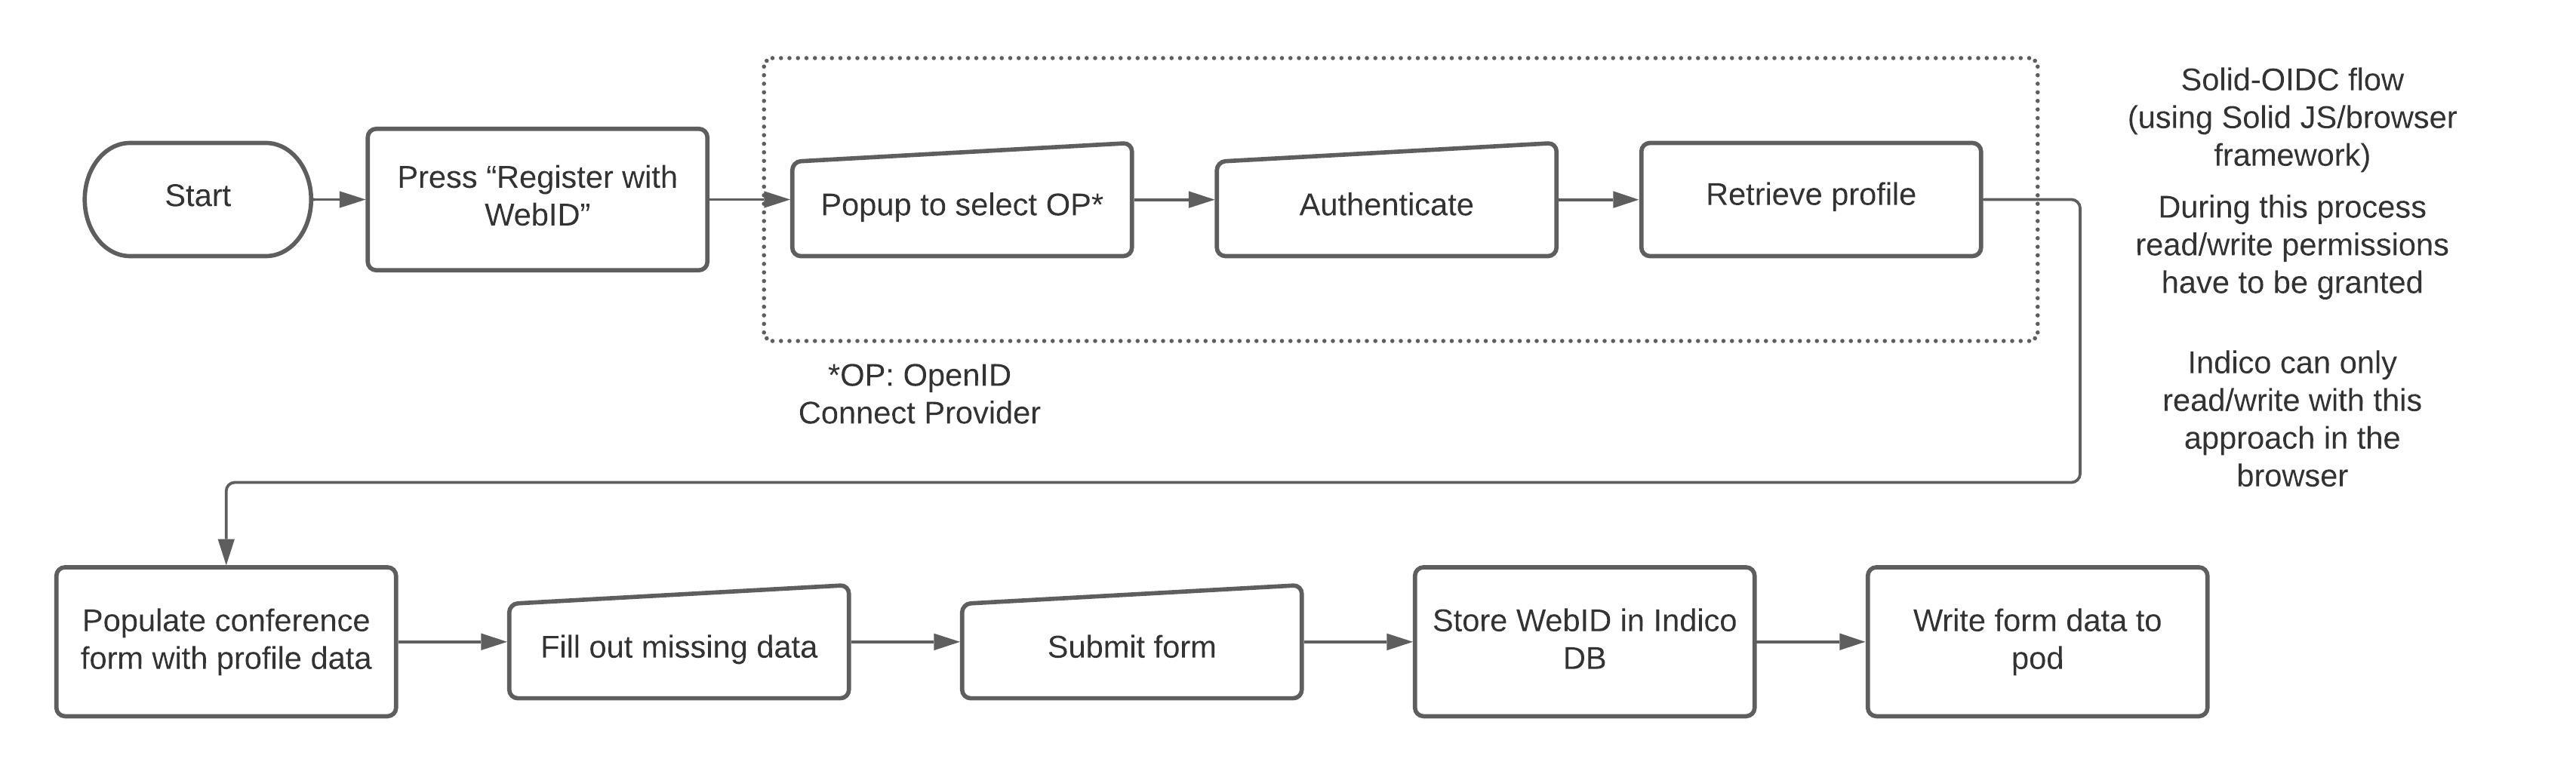
\includegraphics[width=0.6\textwidth]{prototype/graphs/poc-conference_registration_flow-client_side-sideways.jpeg}
    \caption{TODO:}
    \label{fig:poc-conference_registration_flow-client_side-sideways}
\end{figure}

\begin{figure}
    \centering
    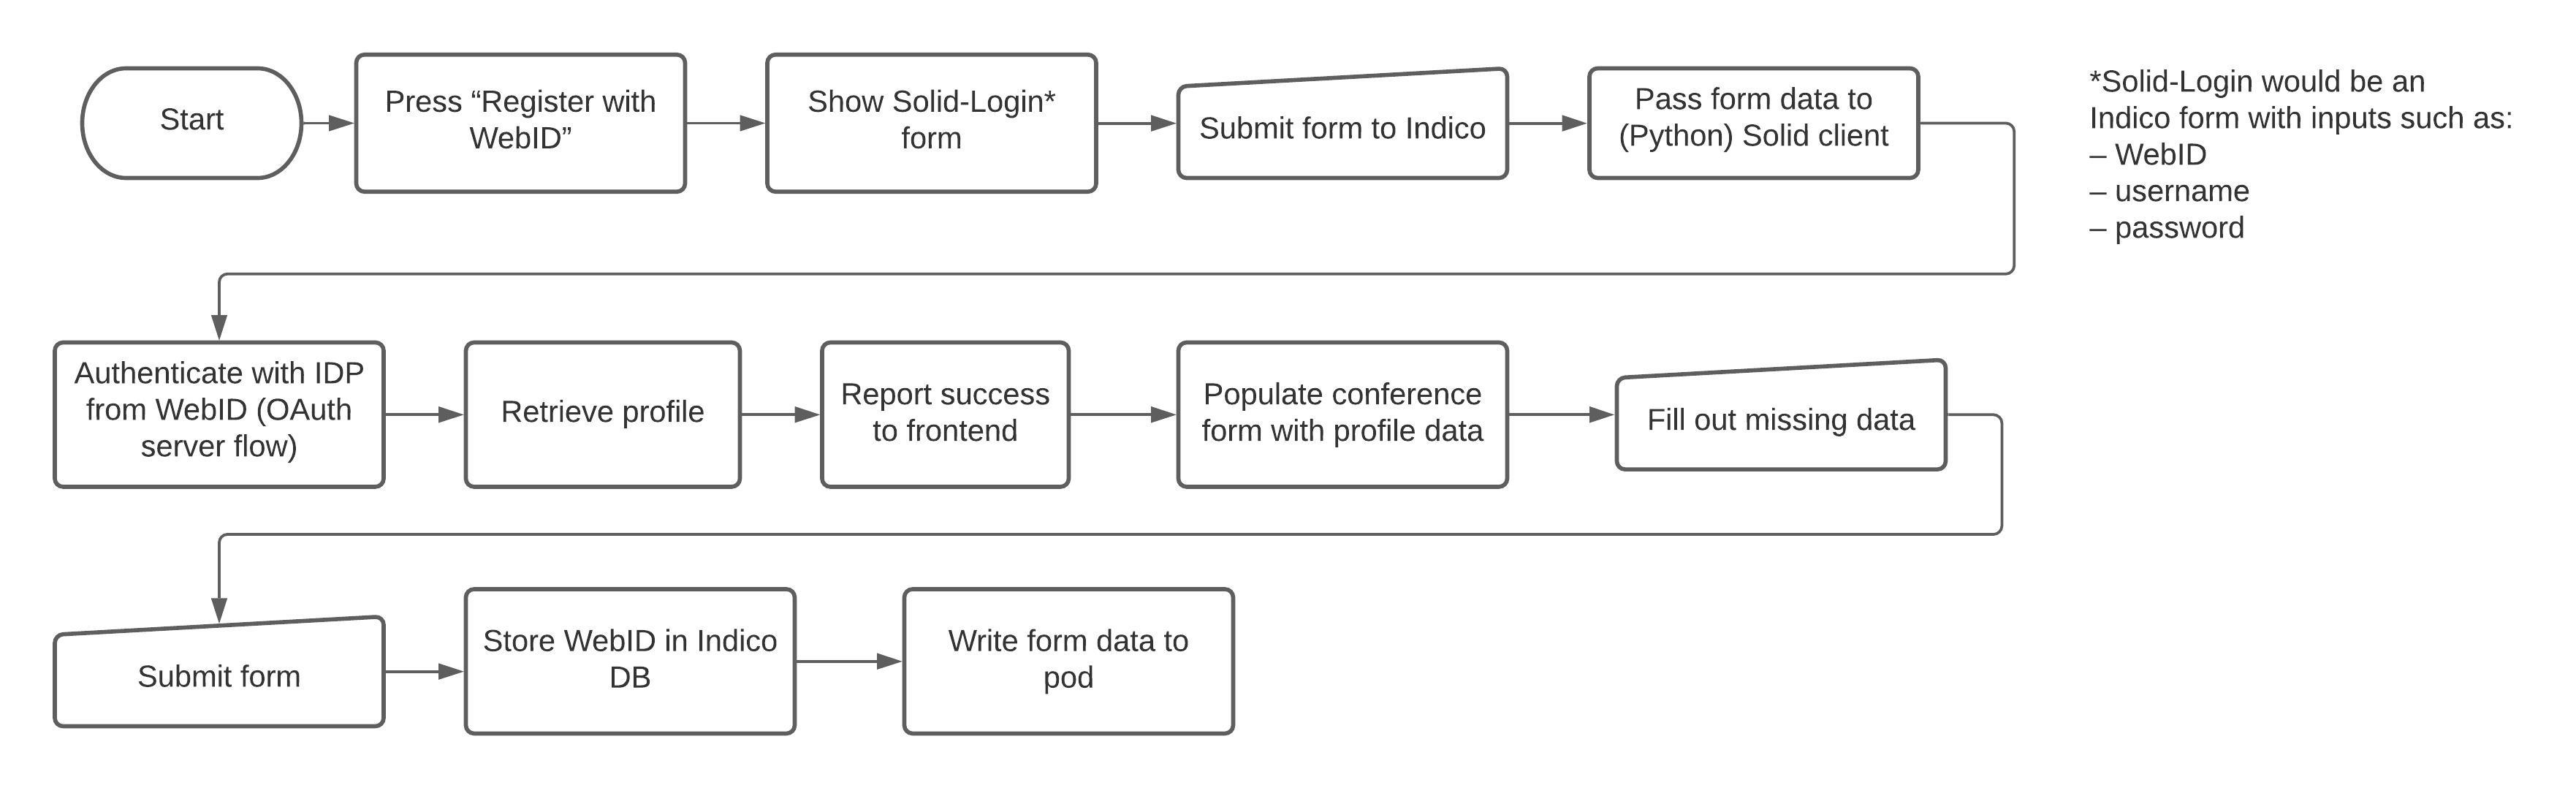
\includegraphics[width=0.6\textwidth]{prototype/graphs/poc-conference_registration_flow-server_side-sideways.jpeg}
    \caption{TODO:}
    \label{fig:poc-conference_registration_flow-server_side-sideways}
\end{figure}

\begin{figure}
    \centering
    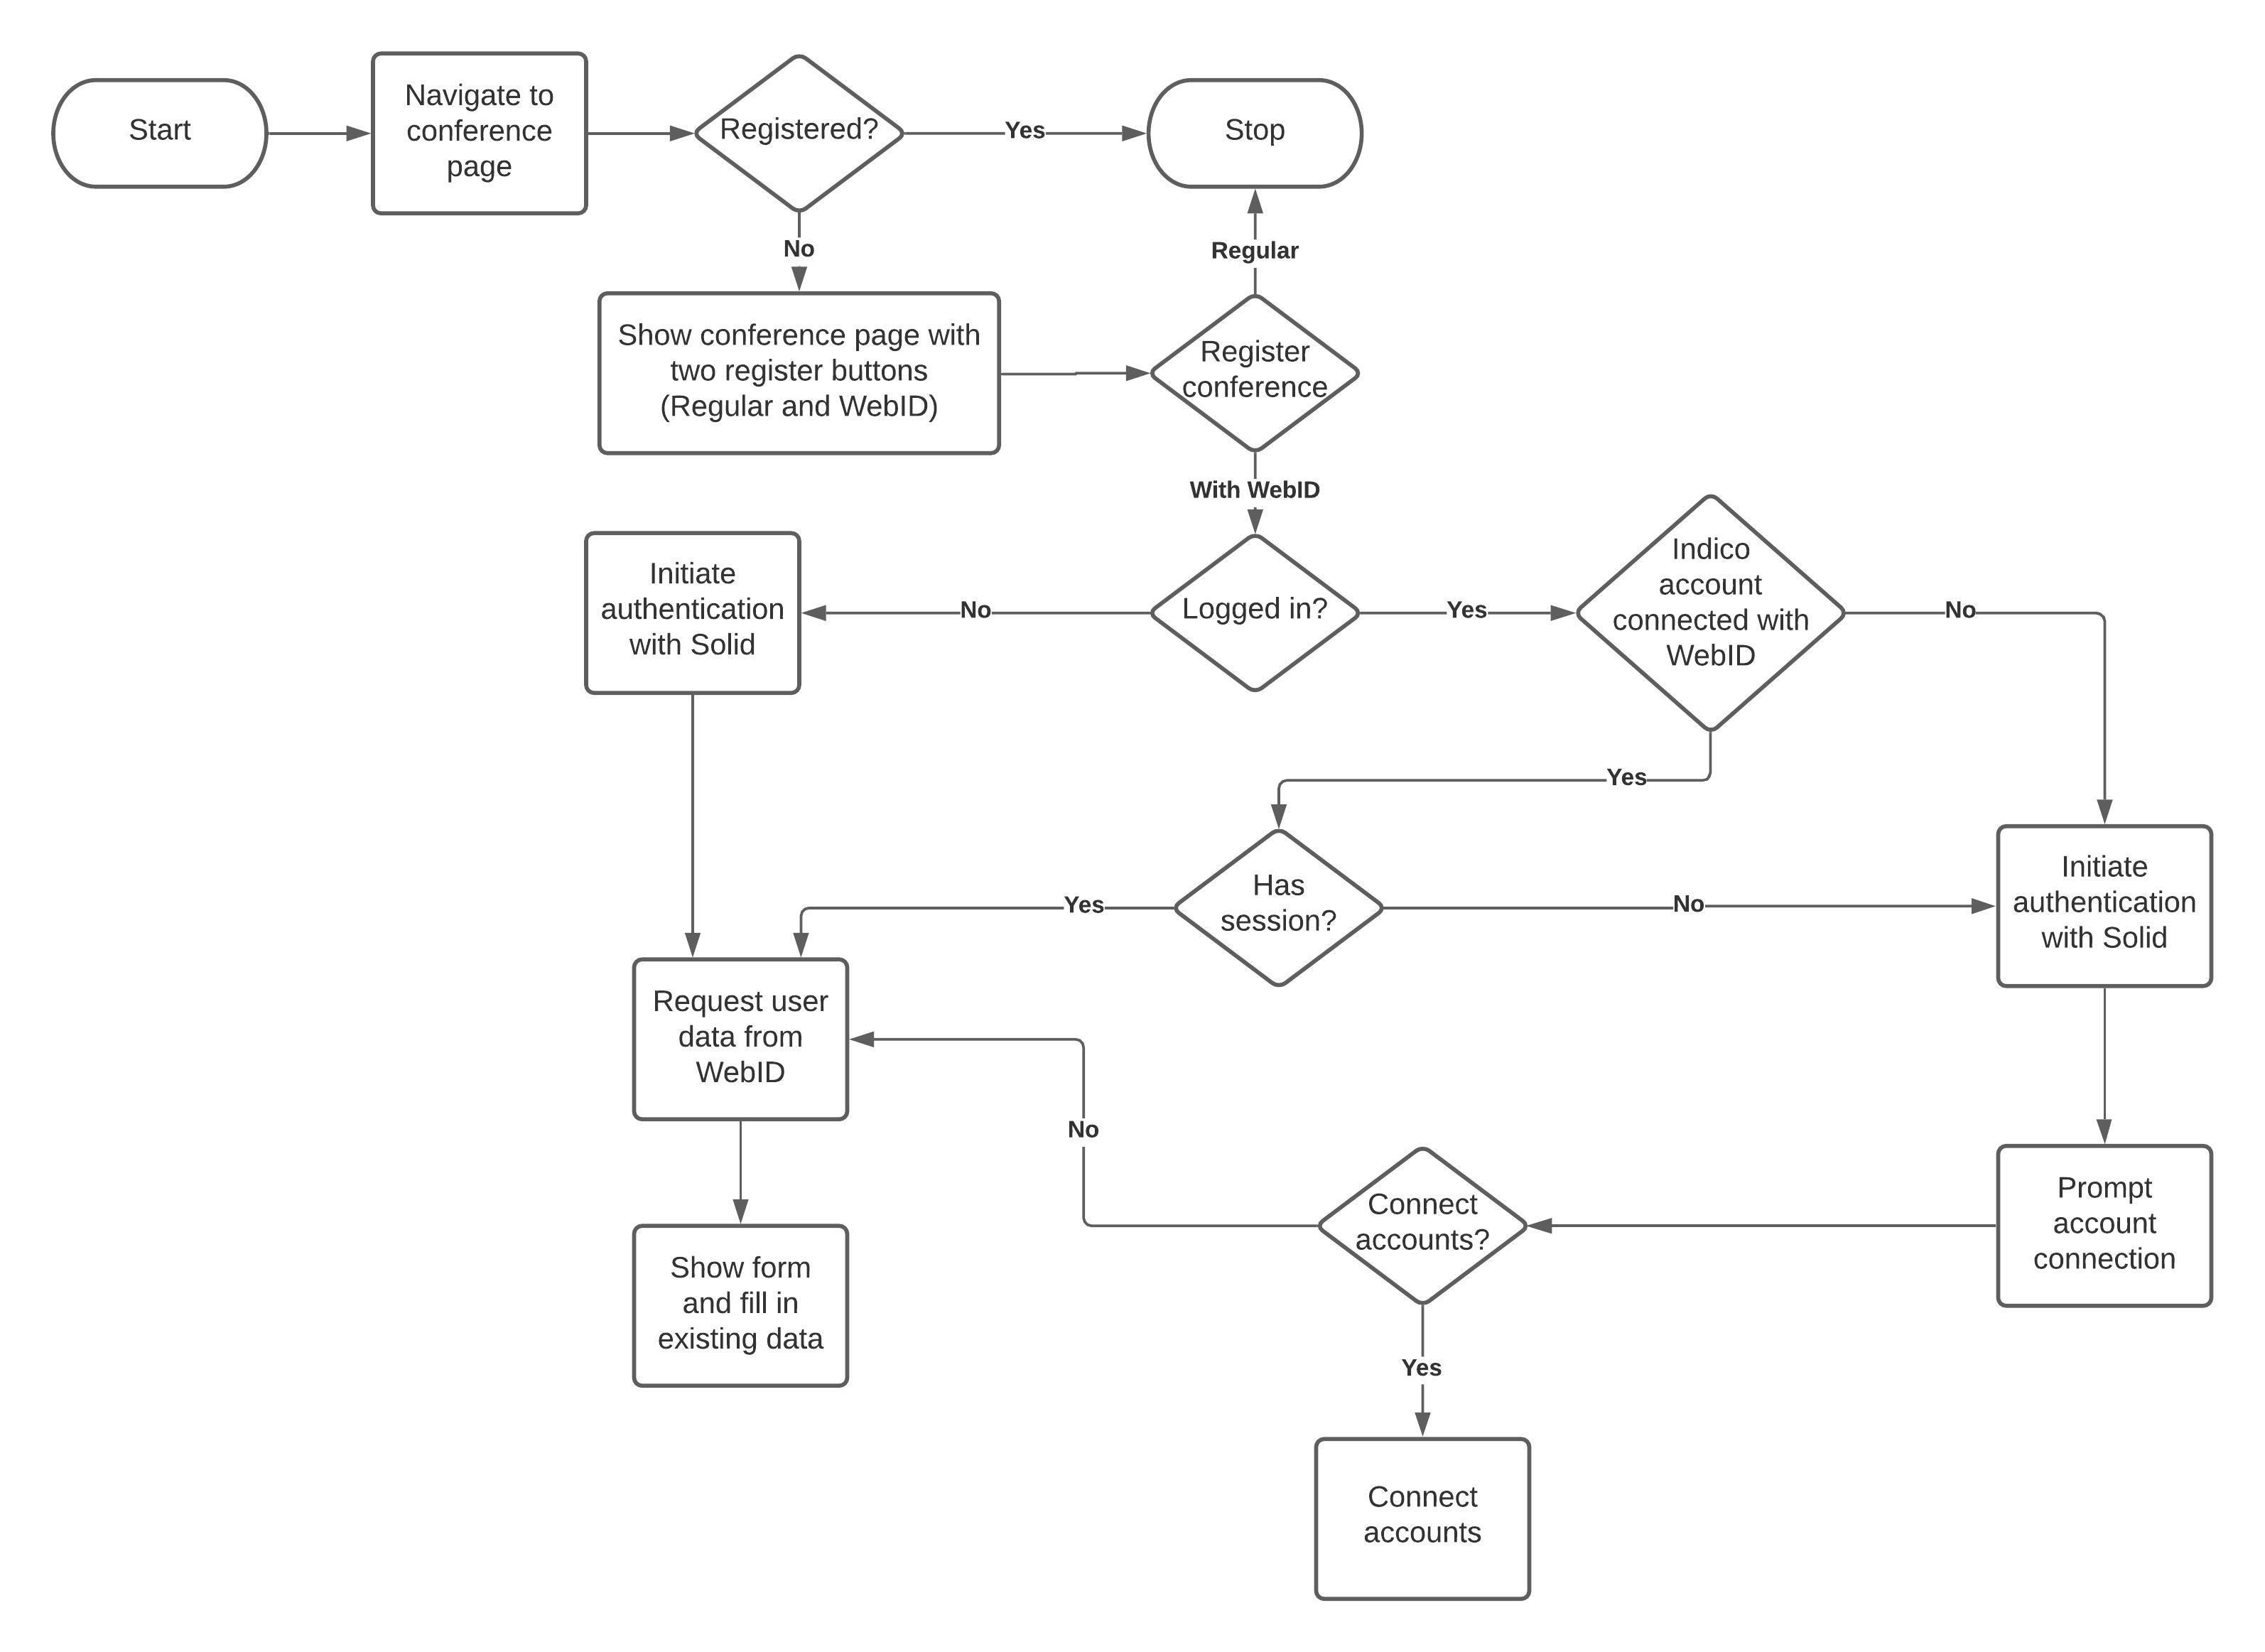
\includegraphics[width=0.6\textwidth]{prototype/graphs/poc-conference_registration_flow-sideways.jpeg}
    \caption{TODO:}
    \label{fig:poc-conference_registration_flow-sideways}
\end{figure}

* Gave up usage control
  * Why it didn't work, and **what is necessary to make it work**
    * usage control
    * question the choice of Indico usage control
    * versioning of tag of personal data
* high-level constraints
* implementation
  * indico limits this
* if indico in this way or more generally

\paragraph{Modification of Resource From Data Pod}\mbox{}\\

\paragraph{Payment on Input Fields}\mbox{}\\

\paragraph{Performance of Large Conference}\mbox{}\\

\paragraph{Availability of Crucial User Data}\mbox{}\\

\subsubsection{Integration With Indico}\mbox{}\\

\paragraph{Bind to Dynamically Created Form}\mbox{}\\

\subsubsection{Evaluation}\mbox{}\\

\paragraph{Metrics}\mbox{}\\
\paragraph{Levels}\mbox{}\\
\paragraph{Components}\mbox{}\\

\subsubsection{Analysis}\mbox{}\\
